\chapter{System Architecture and Methodology}
\label{chap:architecture}
\noindent \rule{6.6in}{0.01in}
\newpage

\section{Overview}

The system is organised as the two-stage pipeline sketched in Figure~\ref{fig:architecture}. Raw event records are cleaned and turned into a fixed set of engineered features (Sections~\ref{sec:dataset}--\ref{sec:feature-engineering}); those features are consumed independently by four base classifiers whose class-probability outputs are combined by a stacked meta-learner into a single severity prediction (Section~\ref{sec:base-classifiers}); and that prediction, together with contextual attributes already known at report time, is passed to a deterministic rule-based engine that produces a concrete resource recommendation (Section~\ref{sec:recommendation-engine}). Section~\ref{sec:inference-pipeline} ties the whole pipeline together into a single inference call, and Section~\ref{sec:fullstack} describes how that call is exposed through a full-stack web application.

\begin{figure}[!h]
\centering
\begin{tikzpicture}[
  node distance = 7mm and 10mm,
  box/.style = {draw, rounded corners, minimum height=0.9cm, minimum width=2.6cm, align=center, font=\small, fill=blue!6},
  stage/.style = {draw, rounded corners, minimum height=0.9cm, minimum width=2.6cm, align=center, font=\small, fill=orange!12},
  outbox/.style = {draw, rounded corners, minimum height=0.8cm, minimum width=2.1cm, align=center, font=\scriptsize, fill=green!8},
  arr/.style = {-{Latex[length=2mm]}, thick}
]
\node[box] (raw) {Historical\\Event Data};
\node[box, right=of raw] (clean) {Cleaning \&\\Imputation};
\node[box, right=of clean] (feat) {Feature\\Engineering};
\node[box, right=of feat] (kmeans) {K-Means\\Clustering};
\node[box, right=of kmeans] (enc) {Encoding \&\\Scaling};

\node[stage, below=of feat, xshift=0.5cm, minimum width=6.6cm] (base) {LightGBM + XGBoost + MLP + TabNet};
\node[stage, below=of base] (meta) {Stacked Meta-Learner (LightGBM)};
\node[box, below=of meta, fill=red!8] (sev) {Severity\\Prediction};
\node[stage, below=of sev, fill=green!12] (rule) {Rule-Based Recommendation Engine};

\node[outbox, below=8mm of rule, xshift=-4.8cm] (o1) {Manpower};
\node[outbox, right=3mm of o1] (o2) {Barricading};
\node[outbox, right=3mm of o2] (o3) {Diversion};
\node[outbox, right=3mm of o3] (o4) {Impact\\Estimate};

\draw[arr] (raw) -- (clean);
\draw[arr] (clean) -- (feat);
\draw[arr] (feat) -- (kmeans);
\draw[arr] (kmeans) -- (enc);
\draw[arr] (enc.south) -- ++(0,-0.35) -| (base.north);
\draw[arr] (base) -- (meta);
\draw[arr] (meta) -- (sev);
\draw[arr] (sev) -- (rule);
\draw[arr] (rule.south) -- ++(0,-0.3) -| (o1.north);
\draw[arr] (rule.south) -- ++(0,-0.3) -| (o2.north);
\draw[arr] (rule.south) -- ++(0,-0.3) -| (o3.north);
\draw[arr] (rule.south) -- ++(0,-0.3) -| (o4.north);
\end{tikzpicture}
\caption{End-to-end system architecture: from raw event data to an operational recommendation.}
\label{fig:architecture}
\end{figure}

\section{Dataset}
\label{sec:dataset}

The dataset is an anonymised export of 8{,}173 historical traffic-event records logged across Bengaluru, with 46 raw attributes covering geographic coordinates, event type and cause, timestamps, corridor and police-jurisdiction identifiers, vehicle information, and resolution/closure details. A column-by-column missingness audit (Figure~\ref{fig:missing}) showed that the 46 raw columns fall into roughly four bands: a handful of columns (\texttt{comment}, \texttt{map\_file}, \texttt{meta\_data}, and several resolution-related fields) are missing in 96--100\% of records and were dropped outright as carrying essentially no signal; a middle band, including \texttt{junction} (69.3\% missing), \texttt{closed\_datetime} (61.6\%), \texttt{zone} (57.9\%), and \texttt{veh\_type} (40.2\%), is missing often enough that dropping it would discard real information, so these columns were retained with an explicit ``unknown'' category or a derived presence flag rather than being imputed as if the value were simply absent; and the remaining columns, including the coordinates, event cause, and priority fields used to build the target, are essentially complete (0\% missing). Pure row identifiers (\texttt{id}, \texttt{client\_id}, \texttt{created\_by\_id}, and similar administrative keys) were dropped regardless of their missingness, since an internal database key carries no geographic or causal signal about severity.

\begin{figure}[!h]
\centering
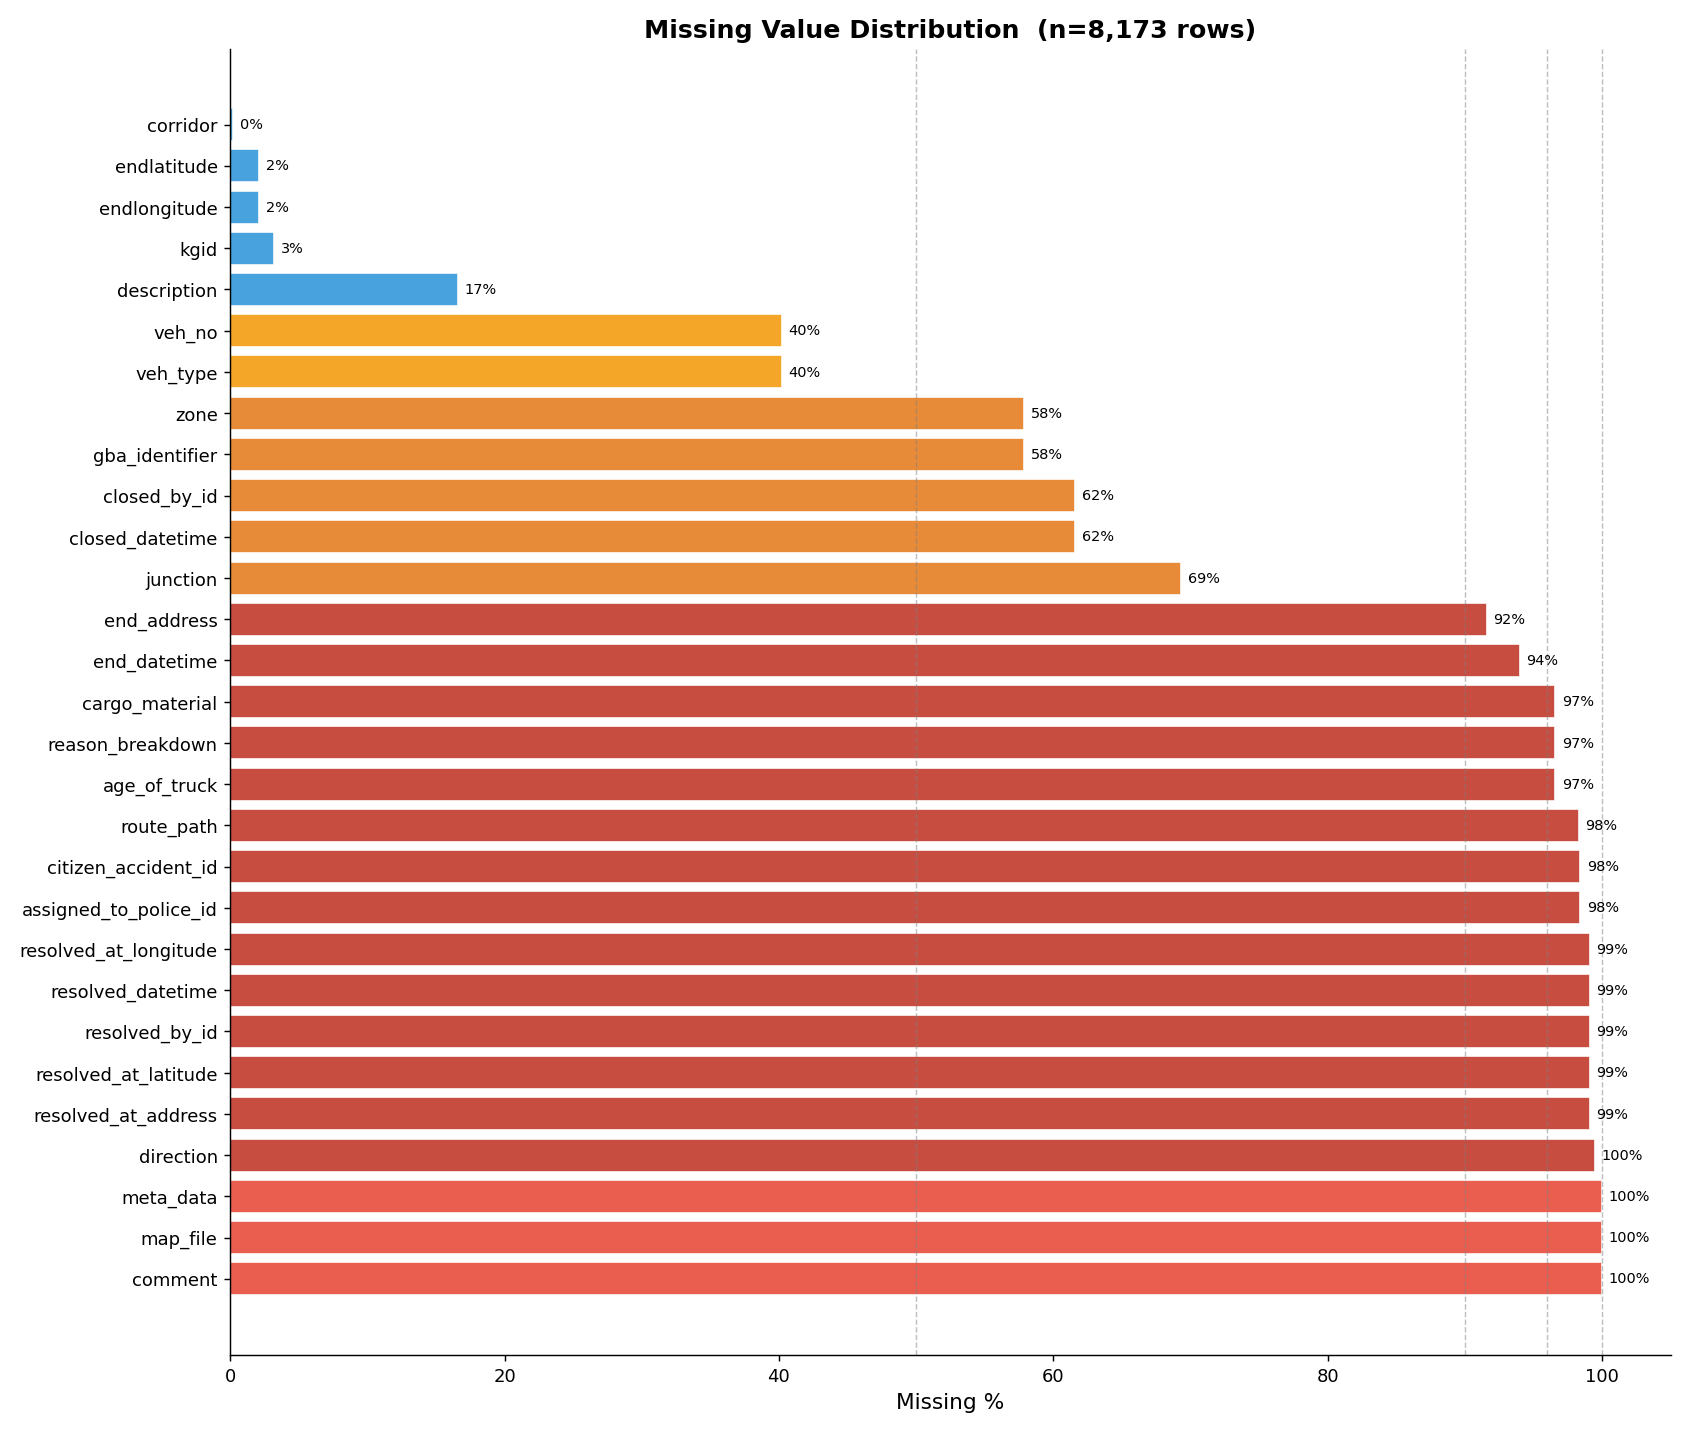
\includegraphics[width=0.85\textwidth]{chapters/5/figs/missing_values.png}
\caption{Missing-value distribution across the 46 raw columns of the event log (n = 8{,}173).}
\label{fig:missing}
\end{figure}

\subsection{Target Variable Construction}
\label{sec:target-construction}

Nowhere in the raw log is there a column that states an event's severity or congestion level directly. The four-class target used throughout this thesis is instead built by combining two fields the control room records independently, for its own operational purposes: the \texttt{priority} tag assigned to the event (High/Low) and whether it \texttt{requires\_road\_closure} (a boolean flag). The four combinations of these two binary fields give a natural four-level ordering, shown in Table~\ref{tab:target-construction}. Both \texttt{priority} and \texttt{requires\_road\_closure} are then removed from the feature set used to train the classifiers -- if they were left in, a model could simply learn the (deterministic) mapping in Table~\ref{tab:target-construction} instead of learning to infer severity from the spatial, temporal, and contextual signals that would actually be available for a genuinely new event.

\begin{table}[!h]
\centering
\caption{Construction of the four-class severity target from two independently recorded fields.}
\label{tab:target-construction}
\begin{tabular}{llcl}
\toprule
Priority & Requires Road Closure & Severity Code & Label \\
\midrule
Low  & No  & 0 & Low \\
Low  & Yes & 1 & Medium \\
High & No  & 2 & High \\
High & Yes & 3 & Critical \\
\bottomrule
\end{tabular}
\end{table}

Table~\ref{tab:class-distribution} and Figure~\ref{fig:target-dist} show the resulting class distribution. The two extreme classes, Low and High, together account for over 91\% of all events, while Medium and Critical make up less than 9\% between them -- Critical events alone are fewer than 300 out of 8{,}173. This confirms, on real data, exactly the imbalance the evaluation methodology in Chapter~\ref{chap:results} is designed around.

\begin{table}[!h]
\centering
\caption{Severity class distribution across all 8{,}173 events.}
\label{tab:class-distribution}
\begin{tabular}{clrr}
\toprule
Code & Label & Count & Percentage \\
\midrule
0 & Low      & 2{,}764 & 33.8\% \\
1 & Medium   &   379   &  4.6\% \\
2 & High     & 4{,}733 & 57.9\% \\
3 & Critical &   297   &  3.6\% \\
\bottomrule
\end{tabular}
\end{table}

\begin{figure}[!h]
\centering
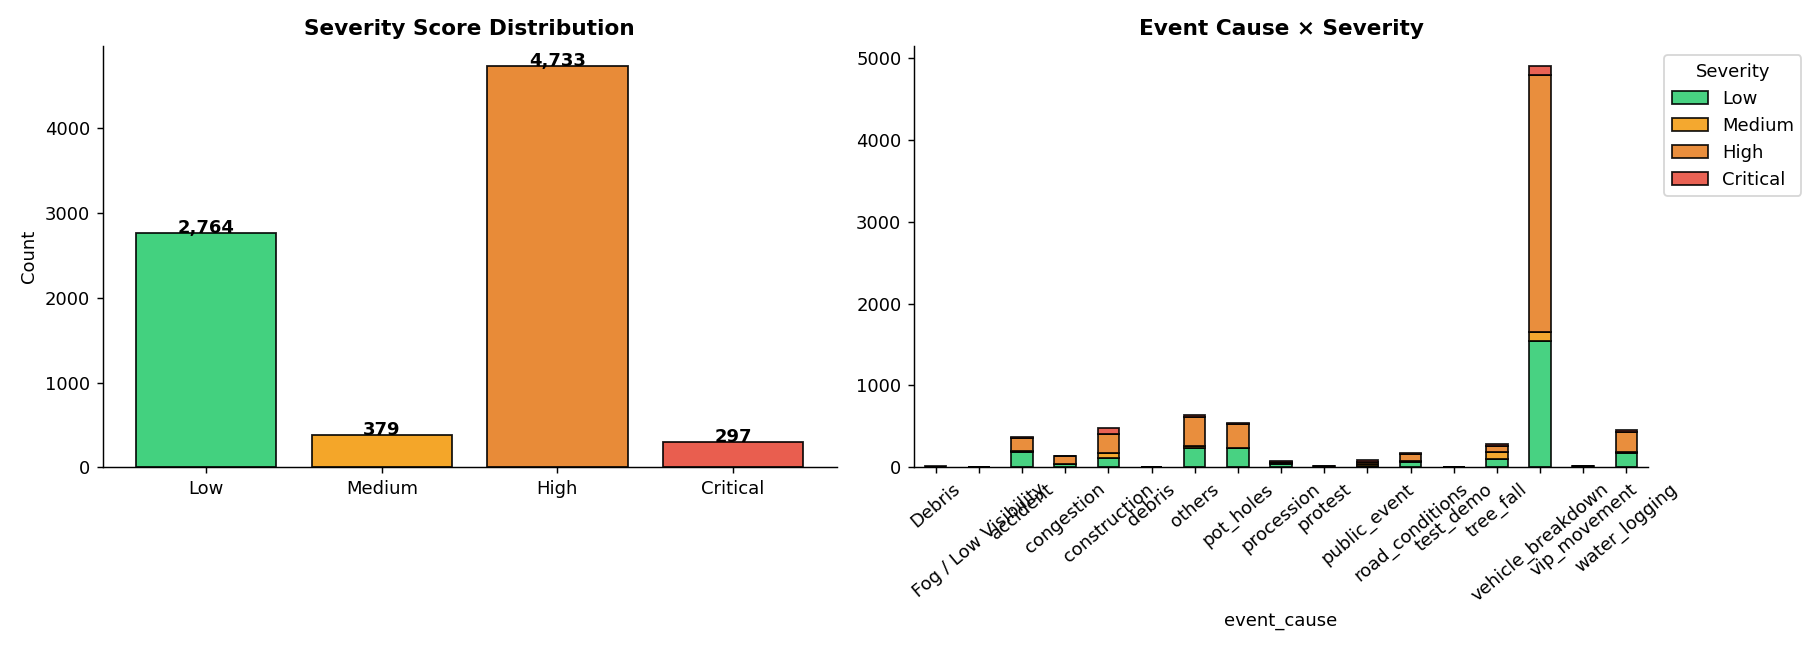
\includegraphics[width=0.95\textwidth]{chapters/5/figs/target_distribution.png}
\caption{Left: severity class counts. Right: how event cause splits across severity levels.}
\label{fig:target-dist}
\end{figure}

\section{Feature Engineering}
\label{sec:feature-engineering}

Thirty features are engineered from the cleaned data and used for modelling, grouped as follows.

\begin{itemize}
\item \textbf{Spatial:} \texttt{latitude}, \texttt{longitude}, \texttt{location\_cluster} (from K-Means, Section~\ref{sec:kmeans}), \texttt{pin\_code} (parsed out of the free-text address field), \texttt{has\_end\_location} (a binary flag, since the raw end-coordinate fields are mostly either genuinely missing or filled with placeholder \texttt{(0, 0)} values that are not real coordinates).
\item \textbf{Temporal:} \texttt{hour}, \texttt{day\_of\_week}, \texttt{month}, \texttt{day}, \texttt{day\_of\_year}, \texttt{is\_weekend}, \texttt{is\_night}, \texttt{is\_morning\_rush} ($7 \le \text{hour} \le 10$), \texttt{is\_evening\_rush} ($17 \le \text{hour} \le 21$), and a coarser \texttt{time\_bucket} category (early morning / morning / afternoon / evening / night / late night).
\item \textbf{Event identity:} \texttt{event\_type}, \texttt{event\_cause}.
\item \textbf{Operational flags:} \texttt{is\_corridor} (whether the event sits on a designated high-density corridor road), \texttt{authenticated\_flag}, \texttt{has\_description}, \texttt{has\_end\_time}, \texttt{has\_been\_closed}.
\item \textbf{Duration / resolution:} \texttt{duration\_mins}, \texttt{resolution\_mins} -- both derived from timestamp differences and clipped to a sensible 0--1440 minute range, with 0 substituted where the underlying timestamp was missing.
\item \textbf{Categorical identifiers:} \texttt{corridor}, \texttt{veh\_type\_simple} (the noisy 40.2\%-null \texttt{veh\_type} field collapsed into five clean buckets -- bus, heavy, private, auto, other/unknown), \texttt{police\_station}, \texttt{zone}, \texttt{junction}, \texttt{status}.
\end{itemize}

After this construction the modelling dataframe has shape $8{,}173 \times 31$ (30 features plus the target), with zero remaining null values. Figure~\ref{fig:correlation} shows each feature's absolute Pearson correlation with the severity target, which is a useful sanity check before training rather than a substitute for the tree-based feature-importance analysis reported later in Section~\ref{sec:feature-importance}.

\begin{figure}[!h]
\centering
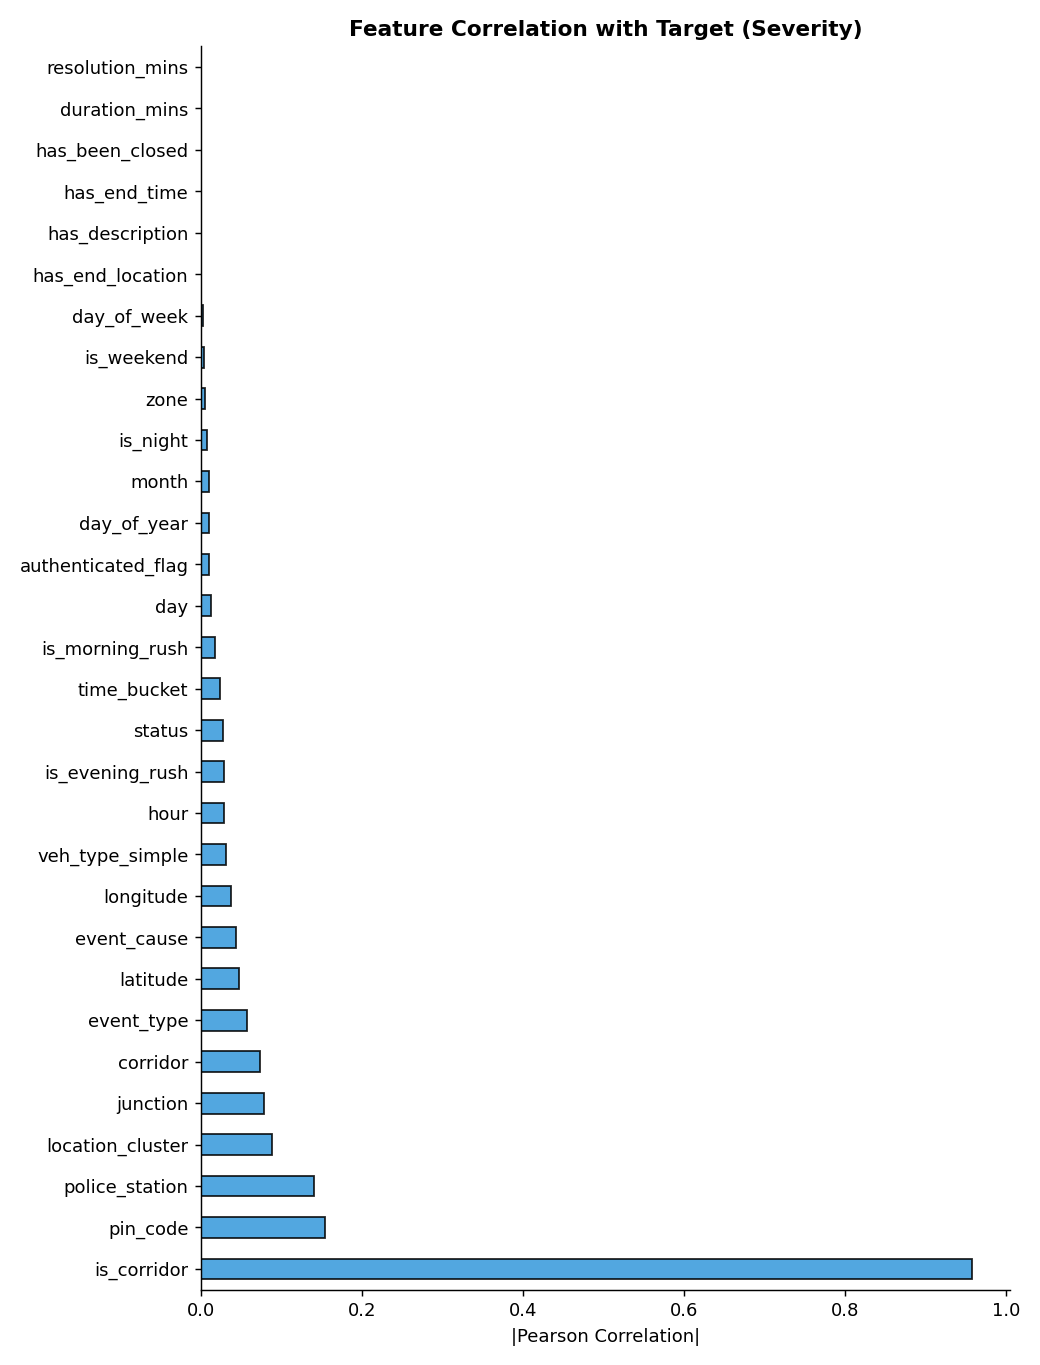
\includegraphics[width=0.7\textwidth]{chapters/5/figs/feature_target_correlation.png}
\caption{Absolute Pearson correlation of each engineered feature with the severity target.}
\label{fig:correlation}
\end{figure}

\subsection{Geographic Clustering with K-Means}
\label{sec:kmeans}

A raw \texttt{(latitude, longitude)} pair on its own gives a classifier very little to generalise from: two events a hundred metres apart have numerically distinct coordinates and are not automatically recognised as belonging to the same neighbourhood. To fix this, the $K$-means clustering algorithm~\cite{macqueen1967methods} is fitted to the event coordinates (using only the 8{,}173 events with valid, non-zero coordinates), with the number of clusters set adaptively as $K = \min(20, \max(5, n/200))$, which for this dataset resolves to $K = 20$. Given $K$ initial centroids, the algorithm alternates between assigning each point to its nearest centroid under Euclidean distance and recomputing each centroid as the mean of its currently assigned points, repeating until the assignment stabilises. The resulting cluster id is stored as \texttt{location\_cluster} and becomes one of the 30 modelling features, letting the downstream classifiers learn region-level severity tendencies -- for instance, a cluster covering a particular high-density corridor experiencing disproportionately more High-severity events -- without needing to memorise raw coordinate values. Figure~\ref{fig:geo-clusters} shows the resulting 20 clusters over Bengaluru.

\begin{figure}[!h]
\centering
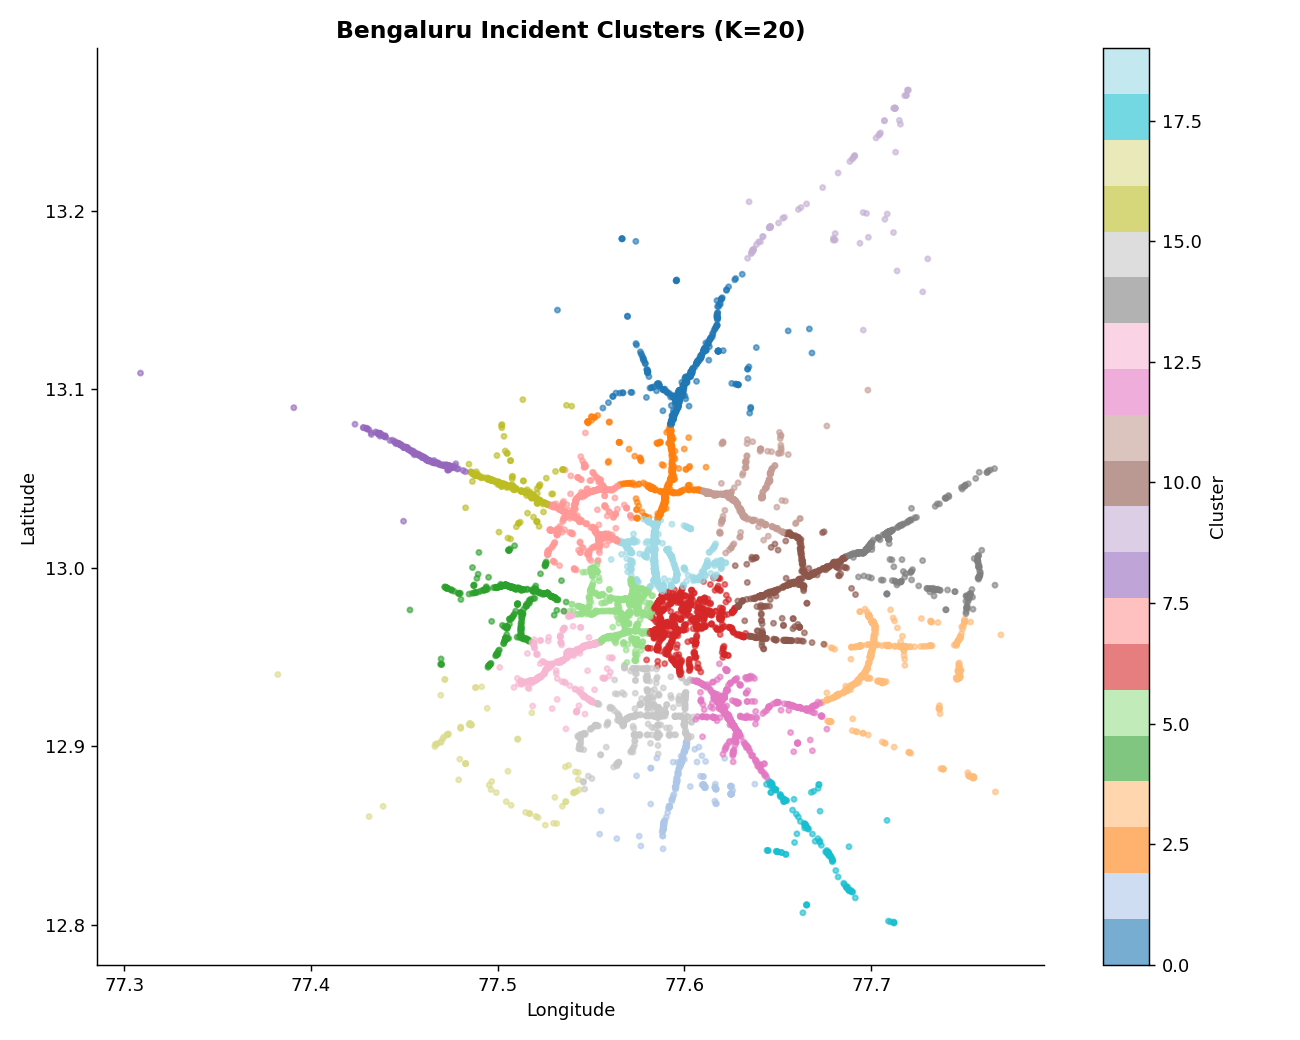
\includegraphics[width=0.65\textwidth]{chapters/5/figs/geo_clusters.png}
\caption{The 20 K-Means geographic clusters fitted over event coordinates across Bengaluru.}
\label{fig:geo-clusters}
\end{figure}

\subsection{Missing-Value Handling and Encoding}

Any numeric column with residual missing values after feature construction is imputed with its column median, which is less sensitive to outliers than the mean. Nine categorical columns -- \texttt{time\_bucket}, \texttt{event\_type}, \texttt{event\_cause}, \texttt{corridor}, \texttt{veh\_type\_simple}, \texttt{police\_station}, \texttt{zone}, \texttt{junction}, \texttt{status} -- are integer-encoded with \texttt{LabelEncoder}, and the fitted encoders are serialized so that the exact same encoding can be reapplied to a new event at inference time (Section~\ref{sec:inference-pipeline}).

\section{Model Training}
\label{sec:base-classifiers}

The 8{,}173 labelled events are split 80/20 into a stratified train/test partition -- 6{,}538 training events and 1{,}635 test events -- preserving the class proportions from Table~\ref{tab:class-distribution} in both splits. Stratification matters here specifically because the Medium and Critical classes are already rare; a plain random split could easily under-represent them further in the test set and make the resulting metrics noisy.

\subsection{Base Classifiers}

Four classifiers are trained independently on the training split.

\begin{itemize}
\item \textbf{LightGBM}~\cite{ke2017lightgbm} -- a histogram-based, leaf-wise gradient-boosted tree ensemble, configured with 1{,}000 estimators, a learning rate of 0.03, 63 leaves, \texttt{feature\_fraction} and \texttt{bagging\_fraction} both at 0.8, balanced class weighting, and L1/L2 regularisation, trained with early stopping (80 rounds) on the held-out test fold.
\item \textbf{XGBoost}~\cite{chen2016xgboost} -- a depth-wise gradient-boosted tree ensemble with 1{,}000 estimators, a learning rate of 0.03, a maximum depth of 6, and row/column sub-sampling of 0.8. XGBoost's scikit-learn interface does not expose a built-in \texttt{class\_weight} option in this configuration, so balanced sample weights are computed explicitly and passed in at fit time; early stopping again uses 80 rounds.
\item \textbf{Multi-Layer Perceptron (MLP)} -- a feed-forward network with hidden layers of size 256, 128, 64, and 32, ReLU activations, and the Adam optimizer~\cite{kingma2015adam}, trained with early stopping (a 15\% validation split, patience of 30 iterations without improvement) to avoid overfitting on a dataset this size. Its inputs are standardised (zero mean, unit variance) before training, since unlike the tree-based models it is sensitive to feature scale.
\item \textbf{TabNet}~\cite{arik2021tabnet} -- an attention-based architecture built specifically for tabular data, configured with a decision/attention embedding width of 32, five sequential decision steps, a sparsity-regularisation coefficient of $10^{-3}$, and the Adam optimizer with a step-decay learning-rate schedule (halving the effective rate roughly every 50 epochs by a factor of 0.9). Training runs for up to 200 epochs with a patience of 30.
\end{itemize}

\subsection{Stacked Ensemble (Meta-Learner)}

Rather than combine the four base models by a simple vote, their class-probability outputs are combined through a stacked ensemble in the sense of Wolpert~\cite{wolpert1992stacked}. To prevent a model's own training data from leaking into the meta-features it later helps predict, out-of-fold (OOF) probabilities are generated with five-fold stratified cross-validation: within each fold, fresh copies of LightGBM, XGBoost, the MLP, and TabNet are trained on the other four folds and used to predict probabilities on the held-out fifth fold. Stacking together the resulting OOF probability vectors -- $4 \times 4 = 16$ dimensions, since each of the four base models outputs a 4-class probability vector -- gives the input to a second LightGBM model, the meta-learner, which learns how much weight to place on each base model's opinion when producing the final severity call.

\section{Rule-Based Resource Recommendation Engine}
\label{sec:recommendation-engine}

A predicted severity code is not, on its own, something a control room can act on -- it still has to be translated into an actual deployment plan. That translation is done by a separate, deterministic rule-based engine, kept intentionally apart from the machine-learning models: the learned models answer ``how severe does this look'', while the rule engine answers ``what do we do about it''. Table~\ref{tab:base-recommendation} gives the base manpower and control-strategy recommendation for each severity level before any contextual adjustment.

\begin{table}[!h]
\centering
\caption{Base severity-to-action mapping used by the recommendation engine.}
\label{tab:base-recommendation}
\small
\begin{tabular}{lp{1.7cm}p{1.4cm}p{4cm}p{4cm}}
\toprule
Severity & Officers (min--max) & Delay est. & Barricading & Diversion \\
\midrule
Low      & 2--4   & 15 min & Cones / indicators only & No diversion needed \\
Medium   & 4--8   & 30 min & Partial barricade (1 lane) + 1 marshal & Advisory alternate route \\
High     & 8--14  & 60 min & Full barricade, both sides, 2 marshal points & Mandatory alternate route + digital signage \\
Critical & 15--25 & 90 min & Full corridor lockdown + marshal chain & Police-escorted diversion + public advisory \\
\bottomrule
\end{tabular}
\end{table}

Two contextual multipliers then adjust this base allocation. If the event is on a designated high-density corridor, the officer range is scaled by $\times 1.4$; if it falls in a peak (rush-hour) window -- 7--10 or 17--21 hours -- the range is scaled by a further $\times 1.25$. Cause-specific rules add extra actions on top of the manpower adjustment: a \texttt{public\_event} of High severity or above triggers a crowd-control-perimeter action and an instruction to coordinate with the event organiser, while an \texttt{accident} of High severity or above triggers an instruction to keep an ambulance lane open and place a trauma centre on standby. For events flagged as pre-announced (planned) rather than sudden, the engine additionally recommends pre-deploying the minimum required officers at least two hours before the event's scheduled start.

\section{Inference Pipeline}
\label{sec:inference-pipeline}

At inference time, a single \texttt{predict\_congestion()} function accepts raw event attributes -- coordinates, event type and cause, start time, corridor and police-station identifiers, vehicle type, expected duration, junction -- and runs the following sequence: (i)~assign the event to its nearest K-Means location cluster; (ii)~construct the same 30 temporal, spatial, and contextual features used in training; (iii)~apply the previously fitted label encoders and standard scaler; (iv)~obtain class probabilities from each of the four base models; (v)~concatenate those probabilities and pass them through the meta-learner to obtain the final severity prediction; and (vi)~pass that prediction, together with event cause, corridor status, and time, to the rule-based recommendation engine to produce the final manpower, barricading, diversion, and delay-estimate output.

\section{Full-Stack Deployment}
\label{sec:fullstack}

The trained pipeline is not left inside the notebook it was developed in -- it is wrapped in a small production-style application so that it can be exercised the way an actual operator would. A Python FastAPI service (the ``ML sidecar'') loads the serialized models, encoders, scaler, and K-Means model once at start-up and exposes the inference pipeline over an internal \texttt{/infer} endpoint. A Go service, built with the Gin framework, sits in front of it as a thin API gateway: it validates incoming requests, forwards them to the sidecar, and exposes the public \texttt{/api/predict}, \texttt{/api/meta}, and \texttt{/api/health} endpoints. A Next.js frontend consumes this API and provides a form for entering an event's details, a Leaflet-based interactive map of Bengaluru, a results view showing the predicted severity, its class-probability breakdown, and the resulting recommendation, and a simple history of past predictions. All three services are containerised and can be brought up together with a single Docker Compose command, which was also the configuration used for deployment (frontend on Vercel, the Go and Python services on Railway).
